\def\COMPLETE{}
\documentclass[11pt]{article}
\usepackage[french, english]{babel}
\usepackage[utf8]{inputenc}
\usepackage{graphicx}
\usepackage{framed}
\usepackage[normalem]{ulem}
\usepackage{amsmath}
\usepackage{amsthm}
\usepackage{amssymb}
\usepackage{amsfonts}
\usepackage{enumerate}
\usepackage{import}
\usepackage[top=1 in,bottom=1in, left=1 in, right=1 in]{geometry}
\usepackage{listingsutf8}
\usepackage{color}
\usepackage{float}
\usepackage{graphicx}
\usepackage{subcaption}
\usepackage[toc,page]{appendix}
\usepackage{multicol}
\usepackage{wrapfig}
\usepackage{sidecap}

\floatstyle{boxed} 
\restylefloat{figure}
\definecolor{mygreen}{rgb}{0,0.6,0}
\definecolor{mygray}{rgb}{0.5,0.5,0.5}
\definecolor{mymauve}{rgb}{0.58,0,0.82}
\newcommand{\dt}{\partial_t}
\newcommand{\Tl}{\frac{T}{\lambda}}
\theoremstyle{definition}
\newtheorem{definition}{Définition}[section]
\DeclareMathOperator*{\argmax}{arg\,max}
\DeclareMathOperator*{\argmin}{arg\,min}
 


\lstset{ 
  backgroundcolor=\color{white},   % choose the background color; you must add \usepackage{color} or \usepackage{xcolor}; should come as last argument
  basicstyle=\footnotesize,        % the size of the fonts that are used for the code
  breakatwhitespace=false,         % sets if automatic breaks should only happen at whitespace
  breaklines=true,                 % sets automatic line breaking
  captionpos=b,                    % sets the caption-position to bottom
  commentstyle=\color{mygreen},    % comment style
  deletekeywords={...},            % if you want to delete keywords from the given language
  escapeinside={\%*}{*)},          % if you want to add LaTeX within your code
  extendedchars=true,              % lets you use non-ASCII characters; for 8-bits encodings only, does not work with UTF-8
  firstnumber=1000,                % start line enumeration with line 1000
  frame=single,	                   % adds a frame around the code
  keepspaces=true,                 % keeps spaces in text, useful for keeping indentation of code (possibly needs columns=flexible)
  keywordstyle=\color{blue},       % keyword style
  language=Python,                 % the language of the code
  morekeywords={*,...},            % if you want to add more keywords to the set
  numbers=left,                    % where to put the line-numbers; possible values are (none, left, right)
  numbersep=5pt,                   % how far the line-numbers are from the code
  numberstyle=\tiny\color{mygray}, % the style that is used for the line-numbers
  rulecolor=\color{black},         % if not set, the frame-color may be changed on line-breaks within not-black text (e.g. comments (green here))
  showspaces=false,                % show spaces everywhere adding particular underscores; it overrides 'showstringspaces'
  showstringspaces=false,          % underline spaces within strings only
  showtabs=false,                  % show tabs within strings adding particular underscores
  stepnumber=2,                    % the step between two line-numbers. If it's 1, each line will be numbered
  stringstyle=\color{mymauve},     % string literal style
  tabsize=2,	                   % sets default tabsize to 2 spaces
  title=\lstname                   % show the filename of files included with \lstinputlisting; also try caption instead of title
}
\lstset{inputencoding=utf8/latin1}
\newcommand{\Dt}{\Delta t}
\newcommand{\Dx}{\Delta x}


\title{\textbf{Dynamique de réseaux multi-échelles complexes sous contraintes: Modélisation et Analyse}}
\author{Liam Toran}
\date{}
\begin{document}
\selectlanguage{french}

\maketitle
\vspace{-20px}
\begin{center}
Stage de fin de M2A 2019 au Laboratoire J.A. Dieudonné de l'Université de Nice\\ sous la supervision d'Yves D'Angelo, Rémi Catellier et Laurent Monasse.
\end{center}
{\footnotesize Thèmes: Mathématiques et leurs Interactions, Modélisation, Analyse, Processus Stochastiques, Équations aux dérivées partielles et ordinaires, Stabilité, Réaction-Diffusion, Ondes progressives, Simulation Numérique.}
\begin{figure}[hb]
\begin{subfigure}[b]{0.5\textwidth}
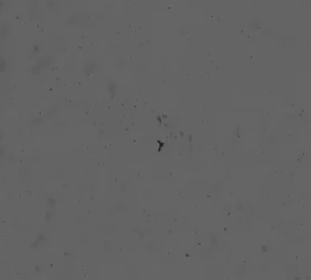
\includegraphics[width=\textwidth]{Images/1.png}
\end{subfigure}
\begin{subfigure}[b]{0.5\textwidth}
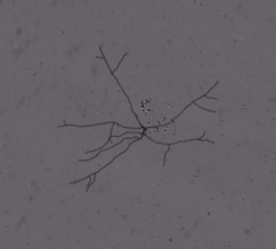
\includegraphics[width=\textwidth]{Images/2.png}
\end{subfigure}
\begin{subfigure}[b]{0.5\textwidth}
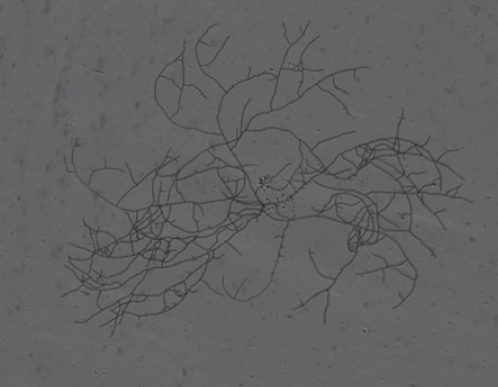
\includegraphics[width=\textwidth]{Images/3.png}
\end{subfigure}
\begin{subfigure}[b]{0.5\textwidth}
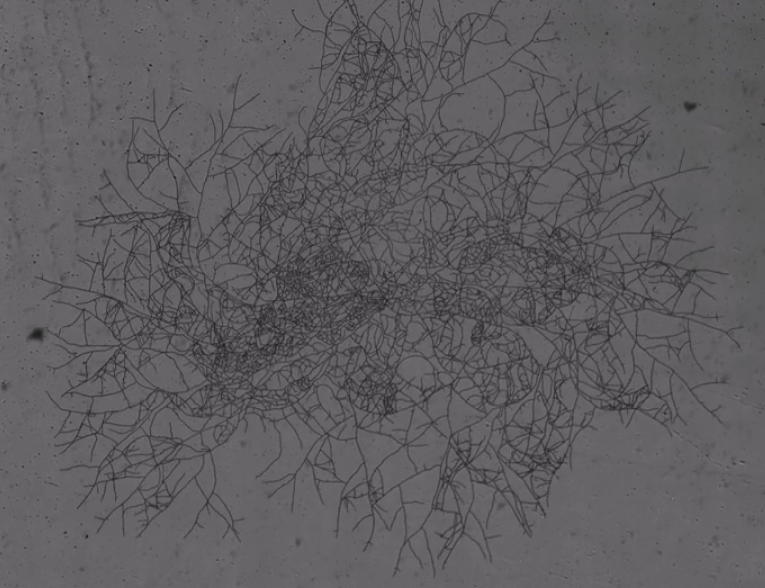
\includegraphics[width=\textwidth]{Images/4.png}
\end{subfigure}
\captionsetup{justification=centering}

\caption{Capture d'un réseau de champignon en expansion, \\ par Éric Herbert, Gwenaël Ruprich-Robert et Florence Leclerc.}
\end{figure}
\newpage
\tableofcontents
\newpage
\setcounter{section}{-1}
\ifdefined\COMPLETE
\else
\documentclass[11pt]{article}
\usepackage[french, english]{babel}
\usepackage[utf8]{inputenc}
\usepackage{graphicx}
\usepackage{framed}
\usepackage[normalem]{ulem}
\usepackage{amsmath}
\usepackage{amsthm}
\usepackage{amssymb}
\usepackage{amsfonts}
\usepackage{enumerate}
\usepackage{import}
\usepackage[top=1 in,bottom=1in, left=1 in, right=1 in]{geometry}
\usepackage{listingsutf8}
\usepackage{color}
\usepackage{float}
\usepackage{graphicx}
\usepackage{subcaption}
\usepackage[toc,page]{appendix}
\usepackage{multicol}
\usepackage{wrapfig}
\usepackage{sidecap}

\floatstyle{boxed} 
\restylefloat{figure}
\definecolor{mygreen}{rgb}{0,0.6,0}
\definecolor{mygray}{rgb}{0.5,0.5,0.5}
\definecolor{mymauve}{rgb}{0.58,0,0.82}
\newcommand{\dt}{\partial_t}
\newcommand{\Tl}{\frac{T}{\lambda}}
\theoremstyle{definition}
\newtheorem{definition}{Définition}[section]
\DeclareMathOperator*{\argmax}{arg\,max}
\DeclareMathOperator*{\argmin}{arg\,min}
 


\lstset{ 
  backgroundcolor=\color{white},   % choose the background color; you must add \usepackage{color} or \usepackage{xcolor}; should come as last argument
  basicstyle=\footnotesize,        % the size of the fonts that are used for the code
  breakatwhitespace=false,         % sets if automatic breaks should only happen at whitespace
  breaklines=true,                 % sets automatic line breaking
  captionpos=b,                    % sets the caption-position to bottom
  commentstyle=\color{mygreen},    % comment style
  deletekeywords={...},            % if you want to delete keywords from the given language
  escapeinside={\%*}{*)},          % if you want to add LaTeX within your code
  extendedchars=true,              % lets you use non-ASCII characters; for 8-bits encodings only, does not work with UTF-8
  firstnumber=1000,                % start line enumeration with line 1000
  frame=single,	                   % adds a frame around the code
  keepspaces=true,                 % keeps spaces in text, useful for keeping indentation of code (possibly needs columns=flexible)
  keywordstyle=\color{blue},       % keyword style
  language=Python,                 % the language of the code
  morekeywords={*,...},            % if you want to add more keywords to the set
  numbers=left,                    % where to put the line-numbers; possible values are (none, left, right)
  numbersep=5pt,                   % how far the line-numbers are from the code
  numberstyle=\tiny\color{mygray}, % the style that is used for the line-numbers
  rulecolor=\color{black},         % if not set, the frame-color may be changed on line-breaks within not-black text (e.g. comments (green here))
  showspaces=false,                % show spaces everywhere adding particular underscores; it overrides 'showstringspaces'
  showstringspaces=false,          % underline spaces within strings only
  showtabs=false,                  % show tabs within strings adding particular underscores
  stepnumber=2,                    % the step between two line-numbers. If it's 1, each line will be numbered
  stringstyle=\color{mymauve},     % string literal style
  tabsize=2,	                   % sets default tabsize to 2 spaces
  title=\lstname                   % show the filename of files included with \lstinputlisting; also try caption instead of title
}
\lstset{inputencoding=utf8/latin1}
\newcommand{\Dt}{\Delta t}
\newcommand{\Dx}{\Delta x}
 %file containing all the used libraries
\begin{document}
\fi

\section{Introduction}


Comment une information ou une rumeur peut être relayée et se propager au sein d'un réseau numérique ou social? Comment un champignon ou une plante envahit un milieu pour y chercher au mieux des substances nutritives? Comment des virus ou des microbes pathogènes peuvent se propager au sein d'une population humaine ou animale? Comment les marchandises, l'énergie, l'argent peuvent circuler de la "meilleure" façon au sein d'une économie? \\
Toutes ces questions semblent se référer à des problématiques sensiblement différentes et à priori étudiées dans des disciplines différentes. L'analyse de ces phénomènes est liée à la dynamique de propagation et diffusion au sein d'un réseau d'agents connectés.  Leur description mathématique repose alors sur des modèles très similaires, qui portent sur la description et la caractérisation d'un nombre croissant d'"individus" en évolution, ainsi que de leurs interactions au sein d'un réseau en expansion spatiale. \\
Le but de ce stage consistait d'une part en l'analyse mathématique des modèles proposés, et d'autre part à développer des approches numériques permettant de simuler et d'analyser la dynamique de ces réseaux. \\
La première section de ce rapport est un rappel de résultats classiques sur les équations de réaction diffusion et en particulier l’équation de Fisher-KPP.\\ La seconde section consiste à l'introduction et l'explication du modèle étudié, le modèle de croissance de réseaux dynamiques branchant, ainsi que l’étude et l'analyse de certaines de ces propriétés. \\ La troisième section expose le calcul de recherche de la vitesse d'onde pour les solutions progressives d'une approximation du modèle.\\ La quatrième section introduit les schémas numériques utilisés pour simuler le modèle approché, ainsi que l'analyse de ces schémas.\\ 
La cinquième expose alors les résultats de la simulation numérique ainsi que l'analyse de ces résultats: notamment, on obtient dans cette partie une validation pour la vitesse d'onde obtenue dans la troisième section. \\
La sixième section revient alors sur le modèle complet (non simplifié) et expose comment retrouver la vitesse d'onde dans ce cas.\\
La septième et dernière section valide ensuite le résultat de la section 6 sur différentes simulations.









\ifdefined\COMPLETE
\else
\end{document}
\fi
\newpage


\section{L'équation de Fisher ou KPP}
\subsection{Préliminaire}
Notre point de départ est l'équation de diffusion:\begin{equation}\dt u = \Delta u  \end{equation}
En plus de la diffusion, considérons des modèles où le taux d'accroissement de $u$ dépend aussi de la densité $u$.\\
Ceci donne les équations de reaction-diffusion:
\begin{equation}\dt u = \Delta u + F(u) \label{eq:ReaDi} \end{equation} 
où F est assez lisse.\\
Il est souvent naturel dans les modèles de considérer $F(u)$ proportionnel à  $u$ pour $u$ petit (``croissance"), et quand $u$ devient proche de 1, l'accroissement $F(u)$ s'arrête: $F(1)=0$ (``saturation").\\
Ces types de modèles ont étés introduits et examinés par les travaux de Fisher[1] %CITER FISHER
et Kolmogorov, Petrovsky et Piscounuv (abrégés KPP).\\ %CITER KPP
Un exemple d'une telle équation est:

\begin{equation}
	\dt u = \Delta u + ru(1-u) \label{eq:KPP}
\end{equation}
où $r>0$, qui sera dans la suite étudiée dans le cas 1-dimensionnel en $x$ : $u=u(x,t)$.

\subsection{Réaction}
En observant les solutions constantes en $x$: $u(x,t)=v(t)$ dans \eqref{eq:KPP}, l'équation différentielle ordinaire (EDO ou ODE): \begin{equation}
	\dt v = r(v - v^2) = F(v)
\end{equation}
est obtenue. \\
Il y a deux équilibres ($F(v)=0)$) pour $v=0$ et $v=1$.Par le théorème de stabilité de Lyapunov, $F'(0)>0$ montre que $v=0$ est instable et $F'(1)<0$ montre $v=1$ est asymptotiquement stable.

\subsection{Réaction-Diffusion}
Dans l’espace $X=C^0_{b,unif}(\mathbb{R},\mathbb{R})$ des fonctions bornées et uniformément continues, il y a existence locale et unicité des solutions de l’équation de Fisher-KPP \eqref{eq:ReaDi}. Grâce à un principe du maximum, il y a aussi existence globale et unicité des solutions.
\newtheorem{theorem}{Théorème}
\begin{theorem}:\\ Existence et Unicité de la solution dans $X$: Soit $U_0 \in X$. Il existe une unique solution de l'équation de Fisher-KPP \eqref{eq:ReaDi}  $U \in C([0,\infty[,X)$ avec condition initiale $U_0$. \end{theorem}
\begin{theorem}:\\ Principe du Maximum: Soit $u_1$ et $u_2$ deux solutions de \eqref{eq:ReaDi}. Si il éxiste $t_0$ tel que $u_1(x,t_0)<u_2(x,t_0) $ $\forall x$ alors $u_1(x,t)<u_2(x,t)$  $ \forall x$ et $\forall t>t_0$ \end{theorem}

\subsection{Solutions en onde plane stationnaire / onde progressive}
Rappellons la définition d'une solution en onde plane stationnaire / onde progressive:
\begin{definition}{Solutions en onde plane stationnaire}\\Une solution en onde plane stationnaire est une solution de la forme $u(x,t)=h(x-st)$ où $c \in \mathbb{R} $.\\ On fera parfois l'abus de notation $u(x,t)=u(x-st)$
\end{definition}
Sous des hypothèses ``faibles" sur $F$, l'équation \eqref{eq:ReaDi}: $\dt u = \Delta u + F(u)$ a alors la propriété surprenante et importante de posséder des solutions en ondes planes stationnaires liant les états d'équilibre $u=1$ (à $-\infty$) et $u=0$ (à $+\infty$).\\
Les hypothèses sur $F$ portent en partie sur le fait que \eqref{eq:ReaDi} doit posséder:\\
- Deux états d'équilibre $u=1$ et $u=0$: $F(0)=F(1)=0$:\\
- Un phénomène de ``croissance" : $F'(0)>0$\\
- Un phénomène de ``saturation" : $F'(1)<0$ \\
\paragraph{Étude des solutions en ondes progressive de \eqref{eq:ReaDi}}:\\
En substituant $u(x,t) = h(x-st) = h(y)$ pour $y=x-st$ dans \eqref{eq:ReaDi}, les équations obtenues sur $h$ sont: \begin{equation} \label{eq:FWS} \left\{
                \begin{array}{ll}
                h''(y)+ sh'(y)+F(h(y))=0 \\
                h(-\infty)= 1 \\  h(+\infty) =0 
                   \end{array}
              \right.
\end{equation} 
qui est une équation elliptique non linéaire. Le problème est donc de trouver $s$ et $h \in C^2$ tels que le système \eqref{eq:FWS} soit vérifié. Le théorème obtenu est le suivant:



\begin{theorem}{\textbf{Existence de solutions en onde progressive pour les équations de reaction-diffusion}}:\\
Soit $F \in C^1([0,1])$ tel $F(0)=F(1)=0$ et $F\geq 0$. \\
Il existe une vitesse critique $s_*$ telle que $s_*^2 \geq 4F'(0)$ et: \\ \\
- i) $\forall s \geq s_*$, l'équation \eqref{eq:FWS} a une solution $h_s:\mathbb{R} \rightarrow ]0,1[$ de classe $C^3$.\\ Cette solution est unique à translation près. \\
- ii)  $\forall s<s_*$ l'équation \eqref{eq:FWS} n'a pas de solution $h:\mathbb{R} \rightarrow [0,1]$
\end{theorem}
\textbf{Remarques}:\\
 Dans le cas ii) il existe des solutions en ondes planes mais elles ne sont pas confinées dans [0,1] ni dans $\mathbb{R}^+$, ce qui ne fait pas de sens dans une étude de densité de population.\\
 Dans le cas de l'équation de Fisher-KPP, c'est à dire pour $F(u)=r(u - u^2)$, on a $s_*^2 = 4F'(0) = 4r $: la vitesse minimale de propagation est $s^* =2\sqrt r $.


\subsection{Théorèmes de sélection de la vitesse pour KPP}
Le théorème important suivant est du aux travaux de Kolmogorov, Petrovsky et Piscounuv de 1937. C'est l'article et le résultat fondateur de la théorie des ondes planes dans les systèmes de réaction-diffusion. %CITER KPP\\

\begin{theorem}{\textbf{Convergence vers une solution d'onde à vitesse minimale pour les solutions de l'équation de Fisher-KPP avec une donnée initiale à support compact }}\\
Soit $u_0 \to ]0,1[$ une donnée initiale à support compact. 
Soit $u$ la solution de l'équation de Fisher-KPP \eqref{eq:KPP} avec $r=1$ et de donnée initiale $u_0$.
Alors quand $t \to \infty$, $u$ converge uniformément en $x$ vers une solution d'onde $h_{s^*}$ de \eqref{eq:FWS} qui se de déplace à vitesse minimale $s^* =2$ :
\begin{equation*}
\sup_{y \in \mathbb{R}}  |u(y+m(t),t)-h_{s^*}(y)| \to_{t\to \infty} 0
\end{equation*}
où $m(t)= 2t - (3/2)\log (t) + y_0 $.
\end{theorem}
Remarque: La vitesse du front est alors $s(t) = \dt m(t) = 2 - \frac{3}{2t} \to_{t\to \infty} 2 $.
\paragraph{}
Ce résultat à été raffiné par la suite par Uchiyama, Bramson et Lau. Leurs travaux apportent plus d'informations sur comment la vitesse du front se sélectionne en fonction de la donnée initiale, et comment il est possible d'obtenir d'autres vitesses de fronts que la vitesse minimale en fonction de la donnée initiale.
\begin{theorem}{\textbf{Sélection de la vitesse pour les solutions de l'équation de Fisher-KPP en fonction de la donnée initiale}}\\
Si $u_0 \to ]0,1[$ vérifie $\lim\inf_{x\to -\infty} u_0(x) > 0$ et $\int_0^{+\infty} xe^xu_0(x) / dx < \infty$\\
alors il existe $y_0 \in \mathbb{R}$ tel que la solution de \eqref{eq:KPP} avec données initiales $u_0$ vérifie
\begin{equation*}
\sup_{y \in \mathbb{R}}  |u(y+m(t),t)-h_{s^*}(y)| \to_{t\to \infty} 0
\end{equation*}
où $m(t)= 2t - (3/2)\log (t) + y_0 $. 
\end{theorem}
D'autres vitesses peuvent être sélectionnées: Si la donnée initiale vérifie $u_0(x) \approx  e^{-\lambda_-(s)x}$ quand $x \to +\infty$ alors la solution converge vers une onde progressive de vitesse $s$.





\newpage
\section{Dyamique de Réseaux en Croissance}
Dans cette section et par la suite nous étudions le modèle sur la croissance de réseaux dynamiques branchant, par exemple un champignon, proposé par Rémi Catellier, Yves D'Angelo et Cristiano Ricci, avec rescaling adéquat:
\begin{equation}\label{eq:BDNG}  \left\{
                \begin{array}{ll}
                \dt\mu + \nabla(\mu v) = f(C)(\mu + \rho) -\mu\rho \\
                   \dt(\mu v)+\nabla(\mu v\times v) +T\nabla\mu=-\lambda\mu v+\mu\nabla C-\mu v \rho \\
                 \dt\rho=  F(v) \mu \\
                  \dt C = -b\rho C
                \end{array}
              \right.
\end{equation} 
L'inconnue $\mu$ représente la densité des apex du champignon.\\
L'inconnue $\rho$ représente la densité des hyphes/ du réseau.\\
L'inconnue $v$ représente la vitesse des apex.\\
L'inconnue $C$ représente la concentration des nutriments.\\
Les paramètres $T$, $\lambda$ et $b$ sont des scalaires représentants la température, l'amortissement fluide sur la vitesse des apex, et le taux de consommation des nutriments par le réseau.\\
La fonction $f$ indique l'influence de la concentration de nutriments sur la croissance du champignon. Pour avoir un état stationnaire sur la croissance du champignon,$f(0)=0$ et $f(x)/x$ dans $L^1$ proche de 0 sont imposés.\\
La fonction $F$ représente l'inverse du temps moyen passé par les apex dans un point donné, et est donné par l'expression:
\begin{equation}
	F(V)=(\frac{1}{2\pi T})^\frac{d}{2}\int_{\mathbb{R}^d} |v|\exp(-\frac{|v-V|^2}{2T})dv\end{equation}
où d est la dimension du problème. Ceci est souvent simplifié en substituant $F(V)$ par une constante: $F(V)= F_0$ .\\

\subsection{Explication des équations du système \eqref{eq:BDNG}}
Le champignon est un réseau branchant dynamique qui peut être étudié en deux parties: les apex (pointes du réseau) représentés par leur densité $\mu$ et les hyphes (branches du réseau) représentés par leur densité $\rho$\\
Les lignes du système \eqref{eq:BDNG} représentent:\\
i) La première ligne du système est le bilan de masse sur les apex avec le terme gauche classique $ \dt\mu + \nabla(\mu v) $. Le terme de droite est composé de : - $f(C)(\mu + \rho)$ correspondant a une croissance proportionnelle à la concentration de nutriments du réseau et la masse existante d'apex et d'hyphes, - et un terme $-\mu\rho$ qui correspond à l'anastomose: une pointe qui rencontre une branche va fusionner avec elle et être détruite. Il y a un terme de croissance et un terme de saturation comme pour le modèle KPP.
\\ ii)  La deuxième ligne est le bilan de vitesse avec le terme de gauche classique $ \dt(\mu v)+\nabla(\mu v\times v) $. Le terme $T\nabla\mu$ représente le mouvement brownien suivi par les apex. Le terme $-\lambda\mu v$ représente un amortissement fluide dans la physique du problème. Le terme  $+\mu\nabla C$ représente la tendance des apex à aller vers les milieux de forte concentration. Le terme $-\mu v \rho $ représente la perte de vitesse du à l'anastomose.\\
iii) La troisième ligne correspond à la relation entre les branches et les pointes: la trace laissée par les apex sont les branches.\\
iv) La quatrième ligne décrit l'évolution de la concentration de nutriments: ils sont consommés par les hyphe avec un taux $bC$ où b est une constante positive.
\subsection{Dérivation de l'équation "KPP avec mémoire"}
En faisant tendre $T$ et $\lambda$ vers $+\infty$, avec $\frac{T}{\lambda}=K$ constant, la deuxième ligne de \eqref{eq:BDNG} donne: 
\begin{equation}
	+K\nabla\mu=-\mu v
\end{equation}
En injectant ceci dans la ligne 1 du système, on obtient le système de 3 inconnues suivant:
 \begin{equation} \left\{
                \begin{array}{ll}
                   \dt\mu = K\Delta\mu + f(C)(\mu + \rho) -\mu\rho\\
                 \dt\rho=  F_0 \mu \\
                  \dt C = -b\rho C
                \end{array}
              \right.
\end{equation}
dit "KPP avec mémoire".
 %1 et 2
\ifdefined\COMPLETE
\else
\documentclass[11pt]{article}
\usepackage[french, english]{babel}
\usepackage[utf8]{inputenc}
\usepackage{graphicx}
\usepackage{framed}
\usepackage[normalem]{ulem}
\usepackage{amsmath}
\usepackage{amsthm}
\usepackage{amssymb}
\usepackage{amsfonts}
\usepackage{enumerate}
\usepackage{import}
\usepackage[top=1 in,bottom=1in, left=1 in, right=1 in]{geometry}
\usepackage{listingsutf8}
\usepackage{color}
\usepackage{float}
\usepackage{graphicx}
\usepackage{subcaption}
\usepackage[toc,page]{appendix}
\usepackage{multicol}
\usepackage{wrapfig}
\usepackage{sidecap}

\floatstyle{boxed} 
\restylefloat{figure}
\definecolor{mygreen}{rgb}{0,0.6,0}
\definecolor{mygray}{rgb}{0.5,0.5,0.5}
\definecolor{mymauve}{rgb}{0.58,0,0.82}
\newcommand{\dt}{\partial_t}
\newcommand{\Tl}{\frac{T}{\lambda}}
\theoremstyle{definition}
\newtheorem{definition}{Définition}[section]
\DeclareMathOperator*{\argmax}{arg\,max}
\DeclareMathOperator*{\argmin}{arg\,min}
 


\lstset{ 
  backgroundcolor=\color{white},   % choose the background color; you must add \usepackage{color} or \usepackage{xcolor}; should come as last argument
  basicstyle=\footnotesize,        % the size of the fonts that are used for the code
  breakatwhitespace=false,         % sets if automatic breaks should only happen at whitespace
  breaklines=true,                 % sets automatic line breaking
  captionpos=b,                    % sets the caption-position to bottom
  commentstyle=\color{mygreen},    % comment style
  deletekeywords={...},            % if you want to delete keywords from the given language
  escapeinside={\%*}{*)},          % if you want to add LaTeX within your code
  extendedchars=true,              % lets you use non-ASCII characters; for 8-bits encodings only, does not work with UTF-8
  firstnumber=1000,                % start line enumeration with line 1000
  frame=single,	                   % adds a frame around the code
  keepspaces=true,                 % keeps spaces in text, useful for keeping indentation of code (possibly needs columns=flexible)
  keywordstyle=\color{blue},       % keyword style
  language=Python,                 % the language of the code
  morekeywords={*,...},            % if you want to add more keywords to the set
  numbers=left,                    % where to put the line-numbers; possible values are (none, left, right)
  numbersep=5pt,                   % how far the line-numbers are from the code
  numberstyle=\tiny\color{mygray}, % the style that is used for the line-numbers
  rulecolor=\color{black},         % if not set, the frame-color may be changed on line-breaks within not-black text (e.g. comments (green here))
  showspaces=false,                % show spaces everywhere adding particular underscores; it overrides 'showstringspaces'
  showstringspaces=false,          % underline spaces within strings only
  showtabs=false,                  % show tabs within strings adding particular underscores
  stepnumber=2,                    % the step between two line-numbers. If it's 1, each line will be numbered
  stringstyle=\color{mymauve},     % string literal style
  tabsize=2,	                   % sets default tabsize to 2 spaces
  title=\lstname                   % show the filename of files included with \lstinputlisting; also try caption instead of title
}
\lstset{inputencoding=utf8/latin1}
\newcommand{\Dt}{\Delta t}
\newcommand{\Dx}{\Delta x}
 %file containing all the used libraries
\begin{document}
\fi



\subsection{Propriétés de l'équation de réaction associée à ``KPP avec mémoire"}
\newtheorem{lemma}{Lemme}
Soit $(\mu,\rho,C)$ vérifiant le système d’équations suivant:
\begin{equation} \left\{
                \begin{array}{ll}
                   \dt\mu  = f(C)(\mu + \rho) -\mu\rho\\
                 \dt\rho=  F_0 \mu \\
                  \dt C = -b\rho C
                \end{array}
              \right.
\end{equation} avec $f(0)=0$. \\
Ce système correspond au systême ``KPP avec mémoire" sans le terme de diffusion.
On s’intéresse au comportement de $(\mu,\rho,C)$ sur $\mathbb{R}^+$ : 
\begin{lemma}$C$ est de signe constant.\\
En effet on a $C(t)= C(0)\exp(-b\int_{0}^{t}\rho(s)ds)$.
\end{lemma}

\begin{lemma}Soit $(\mu,\rho,C)$ tel que $(\mu(0),\rho(0))> (0,0)$ (les deux positifs, au moins un non nul), $C(0)>0$.\\  Alors $\mu(t)\geq 0$ $\forall t>0$.
\end{lemma}
\begin{proof}
Supposons par l'absurde que $\mu$ devient négatif alors soit $t^*= \inf(t>0/ \mu(t)<0)$. Alors: \\
$\mu(t)\geq 0$ $\forall t \leq t^*$\\
$\dt\mu(t^*) \leq 0$ par définition de $t^*$. (Sinon $\mu(t^*+\epsilon)>0$ $\forall \epsilon <<1$)\\
$\rho(t)>0$ $\forall t\leq t^*$ car $\dt\rho=  F_0 \mu$ et $F_0>0$\\
$\dt\mu(t^*) = f(C(t^*))\rho(t^*) > 0$ ce qui est en contradiction avec la deuxième affirmation.
\end{proof}
Dans la suite on se place dans le cas où $(\mu(0),\rho(0))> (0,0)$, $C(0)>0$:
\begin{lemma}
 $\rho$ est croissante car $\dt\rho=  F_0 \mu \geq 0$. En particulier $\rho$ est positive.
\end{lemma}



\begin{lemma}$C$ est décroissante et $\underset{t\to+\infty} \lim C(t) = 0$ \end{lemma}
\begin{proof}$\rho$ est positive donc $C$ est décroissante.\\
 $(\mu(0),\rho(0))> (0,0)$ et $\dt\rho=  F_0 \mu$ impliquent qu'il existe un $t_0$ tel que $\rho(t_0)>0$.\\ Comme $\rho$ est croissante $\forall t\geq t_0$, $\rho(t) \geq \rho(t_0)$.\\Donc $\forall t\geq t_0$, $0<C(t)= C(0)\exp(-b\int_{0}^{t}\rho(s)ds) \leq C_{ste}e^{-b \rho(t_0)t}\underset{t\to+\infty}{\longrightarrow}0$ \\
Donc $\underset{t\to+\infty} \lim C(t) = 0$.
\end{proof}

\newpage 


\begin{lemma} Si $f$ est croissante et  $\int_0^1 \frac{f(x)}{x} dx < \infty $ alors $\mu$ est bornée. \end{lemma}
\begin{proof} On a $\dt\mu  = f(C)(\mu + \rho) -\mu\rho \leq f(C)\mu + f(C)\rho$.
\\
Montrons que $f(C)$ est intégrable:
\\
$C(t)\leq C_{ste}e^{-b \rho(t_0)t}$ et $f$ est croissante donc $\int_0^\infty f(C)dt \leq \int_0^\infty f(C_{ste}e^{-b \rho(t_0)t})dt$.
\\
Soit le changement de variable $u= C_{ste}e^{-b \rho(t_0)t}$, $du = -b\rho(t_0)u\ dt$:
\\
$\int_0^\infty f(C_{ste}e^{-b \rho(t_0)t})dt = \frac{1}{b\rho(t_0)} \int_0^1 \frac{f(u)}{u} du < \infty$ car $\int_0^{C_{ste}} \frac{f(x)}{x} dx < \infty $ donc $f(C)$ est intégrable.
\\
Montrons que $\phi=f(C)\rho$ est intégrable:\\
Effectuons le changement de variable $u = C$, $du = -b\rho u \ dt$ dans $\int_0^\infty f(C) \rho \ dt$:
\\
$\int_0^\infty f(C) \rho \ dt = \frac{1}{b\rho(t_0)} \int_0^{C_{ste}} \frac{f(u)}{u} du  < \infty$ car $\int_0^{C_{ste}} \frac{f(x)}{x} dx < \infty $ donc $\phi = f(C)\rho$ est intégrable.
\\
On a $\dt\mu  \leq f(C)\mu + \phi$.\\
Par le lemme de Gronwall:\\
$\mu(t) \leq \mu(0) + \int_0^t \phi(s) \ ds+\int_0^t \phi(s)f(C)(s)\exp(\int_s^t f(C)(u)du)\ ds \\
 \leq \mu(0) + \int_0^{+\infty} \phi(s) \ ds+ \int_0^t \phi(s)f(C)(s)\exp(\int_0^{+\infty} f(C)(u)du)\ ds \\
 \leq  \mu(0) + \int_0^{+\infty} \phi(s) \ ds+ \exp(\int_0^{+\infty} f(C)(u)du)  \int_0^t \phi(s)f(C)(s) \ ds$\\
$f(C)$ est bornée et  $\phi$ est intégrable donc $f(C)\phi$ est intégrable.\\
On a donc:
$\mu(t) \leq  \mu(0) + \int_0^{+\infty} \phi(s) \ ds+ \exp(\int_0^{+\infty} f(C)(u)du)  \int_0^{+\infty} \phi(s)f(C)(s) \ ds$ $\forall t$
\end{proof}

Dans la suite on se place dans le cas où $f$ est croissante et   $\int_0^1 \frac{f(x)}{x} dx < \infty $
\begin{lemma} $\underset{t\to+\infty} \lim \mu = 0$ \  et $\underset{t\to+\infty} \lim \rho =\rho_\infty < +\infty $ \end{lemma}
\begin{proof}
$\mu$ est bornée, soit $\mu_n$ une suite extraite de la fonction $\mu$ qui tend vers $\ell$.\\
On a $ \ell- \mu(t) = \underset{n\to+\infty} \lim \int_t^{t_n}\dt \mu \ ds = \underset{n\to+\infty} \lim \int_t^{t_n} f(C)(\mu+\rho)-\mu\rho \ ds$.\\
Or $f(C)$ est intégrable (c.f. preuve du lemme 5) et $\mu$ est bornée donc $f(C)\mu$ est intégrable.\\
De même $ f(C)\rho$ est intégrable (c.f. preuve du lemme 5).\\
On a donc $\underset{n\to+\infty} \lim \int_t^{t_n} \mu\rho =  \int_t^{+\infty}(f(C)\mu + f(C)\rho) \ dt \ + \ell -\mu(t) $\\
Or $\mu\rho= F_0\rho\dt\rho = \frac{F_0}{2}\dt \rho ^2$ donc $\int_t^{t_n} \mu\rho \ dt= \frac{F_0}{2}( \rho(t_n) ^2 -\rho(t)^2)$. \\
Or $\rho$ est croissante donc a une limite dans $[0,+\infty]. \\
$Ainsi $\ell$ est déterminée entièrement par la limite de $\rho$ et ne dépend pas de la suite extraite.\\
Par critère séquentiel $\mu$ a une limite $\ell$ qui est finie car $\mu$ est bornée.\\
Mais alors  $\underset{t\to+\infty} \lim \frac{F_0}{2}( \rho(t) ^2 -\rho(T)^2) = \int_T^{\infty}(f(C)\mu + f(C)\rho) \ dt \ + \ell -\mu(T) < \infty$.\\
Donc $\rho^2$ a une limite finie et donc $\rho$ aussi.\\
Comme $\mu = \frac{\dt \rho}{F_0}$ et $\rho$ a une limite finie et $\mu$ aussi, $\mu$ tend nécessairement vers 0. 	 
\end{proof}


\ifdefined\COMPLETE
\else
\end{document}
\fi %2.3
\newpage
\ifdefined\COMPLETE
\else
\documentclass[11pt]{article}
\usepackage[french, english]{babel}
\usepackage[utf8]{inputenc}
\usepackage{graphicx}
\usepackage{framed}
\usepackage[normalem]{ulem}
\usepackage{amsmath}
\usepackage{amsthm}
\usepackage{amssymb}
\usepackage{amsfonts}
\usepackage{enumerate}
\usepackage{import}
\usepackage[top=1 in,bottom=1in, left=1 in, right=1 in]{geometry}
\usepackage{listingsutf8}
\usepackage{color}
\usepackage{float}
\usepackage{graphicx}
\usepackage{subcaption}
\usepackage[toc,page]{appendix}
\usepackage{multicol}
\usepackage{wrapfig}
\usepackage{sidecap}

\floatstyle{boxed} 
\restylefloat{figure}
\definecolor{mygreen}{rgb}{0,0.6,0}
\definecolor{mygray}{rgb}{0.5,0.5,0.5}
\definecolor{mymauve}{rgb}{0.58,0,0.82}
\newcommand{\dt}{\partial_t}
\newcommand{\Tl}{\frac{T}{\lambda}}
\theoremstyle{definition}
\newtheorem{definition}{Définition}[section]
\DeclareMathOperator*{\argmax}{arg\,max}
\DeclareMathOperator*{\argmin}{arg\,min}
 


\lstset{ 
  backgroundcolor=\color{white},   % choose the background color; you must add \usepackage{color} or \usepackage{xcolor}; should come as last argument
  basicstyle=\footnotesize,        % the size of the fonts that are used for the code
  breakatwhitespace=false,         % sets if automatic breaks should only happen at whitespace
  breaklines=true,                 % sets automatic line breaking
  captionpos=b,                    % sets the caption-position to bottom
  commentstyle=\color{mygreen},    % comment style
  deletekeywords={...},            % if you want to delete keywords from the given language
  escapeinside={\%*}{*)},          % if you want to add LaTeX within your code
  extendedchars=true,              % lets you use non-ASCII characters; for 8-bits encodings only, does not work with UTF-8
  firstnumber=1000,                % start line enumeration with line 1000
  frame=single,	                   % adds a frame around the code
  keepspaces=true,                 % keeps spaces in text, useful for keeping indentation of code (possibly needs columns=flexible)
  keywordstyle=\color{blue},       % keyword style
  language=Python,                 % the language of the code
  morekeywords={*,...},            % if you want to add more keywords to the set
  numbers=left,                    % where to put the line-numbers; possible values are (none, left, right)
  numbersep=5pt,                   % how far the line-numbers are from the code
  numberstyle=\tiny\color{mygray}, % the style that is used for the line-numbers
  rulecolor=\color{black},         % if not set, the frame-color may be changed on line-breaks within not-black text (e.g. comments (green here))
  showspaces=false,                % show spaces everywhere adding particular underscores; it overrides 'showstringspaces'
  showstringspaces=false,          % underline spaces within strings only
  showtabs=false,                  % show tabs within strings adding particular underscores
  stepnumber=2,                    % the step between two line-numbers. If it's 1, each line will be numbered
  stringstyle=\color{mymauve},     % string literal style
  tabsize=2,	                   % sets default tabsize to 2 spaces
  title=\lstname                   % show the filename of files included with \lstinputlisting; also try caption instead of title
}
\lstset{inputencoding=utf8/latin1}
\newcommand{\Dt}{\Delta t}
\newcommand{\Dx}{\Delta x}
 %file containing all the used libraries
\begin{document}
\fi

\section{Recherche de la vitesse d'onde des solutions progressives de l’Équation KPP avec Mémoire}
On a le modèle suivant: 
\begin{equation} \left\{
                \begin{array}{ll}
                   \dt\mu -\frac{T}{\lambda}\Delta\mu = f(C)(\mu + \rho) -\mu\rho\\
                 \dt\rho=  F_0 \mu \\
                  \dt C = -b\rho C
                \end{array}
              \right.
\end{equation} 
où $f(0)=0$ et $f$ est positive. Typiquement, $f(C)=C$:\\
Dans la suite on pose $K= \frac{T}{\lambda}$\\
On recherche des solutions en onde plane, on pose $s$ la vitesse d'onde et $\xi = x - st$. \\
\begin{equation} \left\{ \begin{array}{ll} -s \mu'-K\mu''=f(C)(\mu+\rho)-\mu\rho \\ -s\rho' = F_0\mu  \\C'=\frac{b\rho C}{s} \end{array}\right.
\end{equation}
Nos états stationnaires sont $(\mu,\rho,C) = \left\{ \begin{array}{ll} (0,0,C_0) \\
 (0,\rho_\infty,0) , \rho_\infty > 0 \end{array} \right.$ 
\subsection{Au voisinage de $(0,0,C_0)$}
Au voisinage de $(0,0,C_0)$ on a, en posant $f(C_0)=f_0$:
\begin{equation} \left\{ \begin{array}{ll} -s \mu'-K\mu''=f_0(\mu+\rho) \\ -s\rho' = F_0\mu   \end{array}\right.
\end{equation} ce qui devient  \begin{equation} \rho''' +\frac{s}{K}\rho''+\frac{f_0}{K}\rho'-\frac{F_0f_0}{Ks}\rho =0 \end{equation} de polynôme caractéristique \begin{equation} P(X)= X^3 +\frac{s}{K}X^2+\frac{f_0}{K}X-\frac{F_0f_0}{Ks} \end{equation}
Pour $s<0$,   $P(0)>0$ donc P a une racine négative $r_1$ .\\
Pour que P ait deux autres racines réelles $r_3>r_2>r_1$ il faut (condition nécessaire et suffisante) que P' s'annule deux fois et que le discriminant $\Delta$ de P soit positif.
\subsubsection{Première condition: P' a deux annulations:}
$P'(X)= 3X^2+ 2\frac{s}{K}X+ \frac{f_0}{K}$ a pour discriminant $\Delta'=4\frac{1}{K^2}(s^2-3Kf_0)$ ce qui donne la condition \begin{equation} \label{eq:condition_P'}
	\boxed{s^2 >3K f_0
	}
\end{equation}
\subsubsection{Deuxième condition: $\Delta>0$:}
Pour $P=aX^3 +bX^2 + cX + d$ on a $\Delta= b^2c^2 +18abcd-27a^2d^2 -4ac^3 -4b^3d$ ce qui dans notre cas donne
\begin{align*}
	\Delta=\frac{1}{K^4}f_0^2s^2 -18 \frac{f_0^2F_0}{K^3}-27 \frac{F_0^2 f_0^2}{K^2s^2} - 4 \frac{f_0^3}{K^3}+4 \frac{F_0f_0s^2}{K^4} \\ = s^2 \frac{f_0(f_0+4F_0)}{K^4}- \frac{f_0^2(18F_0+4)}{K^3} -\frac{27F_0^2f_0^2}{K^2} \frac{1}{s^2}\\ 
=	\frac{f_0}{K^4s^2}[(f_0+4F_0)s^4-Kf_0(18F_0+4) s^2 - 27 K^2F_0^2f_0] \end{align*}
On est revenu à étudier le signe du polynôme en $s^2$ \begin{equation}
	D(s^2)=(f_0+4F_0)s^4-Kf_0(18F_0+4)s^2 - 27 K^2F_0^2f_0
\end{equation} 
de discriminant $d$:
\begin{align*}
	d=\Big(Kf_0(18F_0+4) \Big)^2 +108(f_0+4F_0)K^2F_0^2f_0 \\ 
	= K^2f_0(f_0(18F_0+4)^2+108(f_0+4F_0)F_0^2) >0
\end{align*}
On obtient donc la condition sur la positivité de $\Delta$: 
\begin{equation}\boxed{
	s^2> K\frac{f_0(18F_0+4)+\sqrt{f_0(f_0(18F_0+4)^2+108(f_0+4F_0)F_0^2)}}{2(f_0+4F_0)}
	}\label{eq:condition_Delta}
\end{equation}
\subsubsection{Signe des racines au voisinage de $(0,0,C_0)$}
On sait déjà que $r_3<0$. Comme $r_1r_2r_3<0$, on remarque que $r_2$ et $r_1$ sont du même signe.\\
De plus $P'$ a un axe de symétrie $X=-\frac{s}{3K}>0$ car $s<0$ donc $P$ atteint un minimum local (forcement négatif) en un point positif donc $P$ a une racine positive.\\
On en déduit $r_1>r_2>0$: \\ 
Sous les conditions \eqref{eq:condition_P'} et \eqref{eq:condition_Delta}, $P$ a deux racines positives et une négative.
\subsection{Au voisinage de $(0,\rho_\infty,0)$} 
Autour de $(0,\rho_\infty,0)$:
Posons $(\mu,\rho,C)=(\mu, \rho_\infty + \epsilon, C)$. On a \\
\begin{equation} \left\{ \begin{array}{ll} -s \mu'-K\mu''=f(C)\rho_\infty-\mu\rho_\infty\\C'=\frac{b\rho_\infty C}{s} \\
-s\epsilon'= F_0\mu \end{array}\right.
\end{equation}
la deuxième ligne donne \begin{equation}
C(y) = \Lambda\exp(\frac{b\rho_\infty}{s}y )
\end{equation}
et la réunion de la première et la deuxième se traduit sur $\epsilon$ par:
\begin{equation}
	s^2 \epsilon''+Ks\epsilon'''=f(C)F_0\rho_\infty+s\epsilon'\rho_\infty
\end{equation} est une EDO d'ordre trois en $\epsilon$ avec terme source $\frac{F_0f(C)}{Ks} \rho_\infty$ de polynôme caracteristique: \begin{equation}
	Q(X)=X^3+\frac{s}{K}X^2-\frac{\rho_\infty}{K}X
\end{equation}
qui possède toujours trois racines:  $0$, une négative et une positive: $X= - \frac{1}{2K}(s \pm \sqrt{s^2+4\rho_\infty Ks})$
Sur $\mu$ on a: \begin{equation}
	-s \mu'-Ks\mu''=f(C)\rho_\infty-\mu\rho_\infty
\end{equation}
Dans le cas $f(C)=C$:\\
$\mu$ a pour polynôme caractéristique homogène $M(X)=X^2 +\frac{1}{K}X - \frac{\rho_\infty}{Ks}$ de racines:\\$r_{1,2}= - \frac{1}{2K}(1 \pm \sqrt{1+4 \frac{\rho_\infty K}{s}})$ \\ donc $\mu_H = Ae^{r_1y}+ Be^{r_2y}$ (On choisit $r_1>r_2$).\\
En cherchant une solution particulière de la forme $\mu_p =M\exp(\frac{b\rho_\infty}{s}y )$ on obtient $M = - \frac{\Lambda}{b^2\rho_\infty K + b - 1}$ et donc $\mu=Ae^{r_1y}+ Be^{r_2y}+M e^{\frac{b\rho_\infty}{s}y }$
et donc $\rho = \rho_\infty + \alpha e^{r_1y} + \beta e^{r_2y} + \Gamma \exp(\frac{b\rho_\infty}{s}y)$ pour $\Gamma = \frac{Ms}{b\rho_\infty} $

\ifdefined\COMPLETE
\else
\end{document}
\fi %3
\newpage
\section{Schémas Numériques}
On a le modèle suivant (``KPP avec mémoire"): 
\begin{equation} \left\{
                \begin{array}{ll}
                   \dt\mu = K\Delta\mu + C(\mu + \rho) -\mu\rho\\
                 \dt\rho=  F_0 \mu \\
                  \dt C = -b\rho C
                \end{array}
              \right.
\end{equation}
\subsection{Pour l'équation différentielle ordinaire}
Sans dépendance spatiale:
\begin{equation} \left\{
                \begin{array}{ll}
                   \dt\mu = C(\mu + \rho) -\mu\rho\\
                 \dt\rho=  F_0 \mu \\
                  \dt C = -b\rho C
                \end{array}
              \right.
\end{equation} 
\subsubsection{Schéma semi-implicite I pour l'EDO}
Soit le schéma semi-implicite I pour l'EDO:
\begin{equation} \boxed{\left\{
                \begin{array}{ll}
                   \mu^{n+1} = \mu^{n}+  \Dt( C^{n}(\mu^{n+1} + \rho^{n+1}) -\mu^{n+1}\rho^{n})\\
                \rho^{n+1}=  \rho^{n}+ \Dt (F_0 \mu^{n+1}) \\
                 C^{n+1} =C^{n}- \Dt(b\rho^{n+1}C^{n+1})
                \end{array}
              \right.}
\end{equation}
Ce schéma donne:
\begin{equation*} \left\{
                \begin{array}{ll}
                   \mu^{n+1}(1-\Dt(C^{n}(1+\Dt F_0)) + \rho^{n}) = \mu^{n}+  \Dt C^{n}\rho^{n} \\
                \rho^{n+1}=  \rho^{n}+ \Dt (F_0 \mu^{n+1}) \\
                 C^{n+1} =C^{n}\frac{1}{1+ \Dt b\rho^{n+1}}
                \end{array}
              \right.
\end{equation*}
\paragraph{Positivité}
Pour conserver la positivité il suffit que le terme $(1-\Dt(C^{n}(1+\Dt F_0)) + \rho^{n}) $ reste positif:\\
Par exemple: 
\begin{equation}
	\boxed{C^0< \frac{1}{\Dt(1+F_0\Dt)}}
\end{equation}

\subsubsection{Schéma semi-implicite II pour l'EDO}
Soit le schéma semi-implicite II pour l'EDO:
\begin{equation} \boxed{\left\{
                \begin{array}{ll}
                   \mu^{n+1} = \mu^{n}+  \Dt( C^{n}(\mu^{n+1} + \rho^{n+1}) -\mu^{n}\rho^{n})\\
                \rho^{n+1}=  \rho^{n}+ \Dt (F_0 \mu^{n+1}) \\
                 C^{n+1} =C^{n}- \Dt(b\rho^{n+1}C^{n+1})
                \end{array}
              \right.}
\end{equation}
Ce schéma donne:
\begin{equation*} \left\{
                \begin{array}{ll}
                   \mu^{n+1}(1-\Dt(C^{n}(1+\Dt F_0))) = \mu^{n}+  \Dt \rho^{n}(C^{n}-\mu^{n}) \\
                \rho^{n+1}=  \rho^{n}+ \Dt (F_0 \mu^{n+1}) \\
                 C^{n+1} =C^{n}\frac{1}{1+ \Dt b\rho^{n+1}}
                \end{array}
              \right.
\end{equation*}
\paragraph{Positivité}
Pour conserver la positivité il suffit que les terme $(1-\Dt(C^{n}(1+\Dt F_0)))$ et $\mu^{n}+  \Dt \rho^{n}(C^{n}-\mu^{n})$ restent positif:\\
Par exemple: 
\begin{equation}
	\boxed{C^0< \frac{1}{\Dt(1+F_0\Dt)}}
\end{equation}
et 
\begin{equation}
	\boxed{\rho^n< \frac{1}{\Dt}}
\end{equation}
On obtient une condition de plus que le schéma semi-implicite I.
\subsection{Pour l'équation aux dérivées partielles}
\subsubsection{Schéma semi-implicite I pour l'EDP}
Soit le schéma semi-implicite I pour l'EDP:
\begin{equation} \boxed{\left\{
                \begin{array}{ll}
                   \mu^{n+1}_i = \mu^{n}_i+ K\Dt \frac{\mu^{n+1}_{i+1}-2\mu^{n+1}_i+\mu^{n+1}_{i-1}}{\Dx ^2} + \Dt( C^{n}_i(\mu^{n+1}_i + \rho^{n+1}_i) -\mu^{n+1}_i\rho^{n}_i)\\
                \rho^{n+1}_i=  \rho^{n}_i+ \Dt (F_0 \mu^{n+1}_i) \\
                 C^{n+1}_i =C^{n}_i- \Dt(b\rho^{n+1}_iC^{n+1}_i)
                \end{array}
              \right.}
\end{equation}
Ce schéma donne:
\begin{equation*} \left\{
                \begin{array}{ll}
                   (1+\frac{K\Dt}{\Dx^2}A-\Dt(C^{n}(1+\Dt F_0)) + \rho^{n})\mu^{n+1} = \mu^{n}+  \Dt C^{n}\rho^{n} \\
                \rho^{n+1}=  \rho^{n}+ \Dt (F_0 \mu^{n+1}) \\
                 C^{n+1} = C^{n}\frac{1}{1+ \Dt b\rho^{n+1}}
                \end{array}
              \right.
\end{equation*}
où $A$ est la matrice de $-\Delta$
:\begin{equation}  \label{myeq}A= \left[ \begin{matrix}2 & -1 & & 0\\-1 & \ddots & \ddots &  \\& \ddots & \ddots &  -1 \\0 &  & -1 & 2  \end{matrix}  \right]\end{equation}
\paragraph{Positivité}
Afin de préserver la positivité, on obtient la même condition (suffisante) que pour l'EDO:
\begin{equation}
	\boxed{C^0< \frac{1}{\Dt(1+F_0\Dt)}}
\end{equation}
\begin{proof} Supposons $\mu^0 >0$.\\ Raisonnons par l'absurde et supposons que $n=\min{n \mid \exists j \mid \mu^{n+1}_j < 0}$ existe. Soit $j = \argmin{\mu^{n+1}_i}$.\\
On a $(1-\Dt(C^{n}_j(1+\Dt F_0)) + \rho^{n}_j)\mu^{n+1}_j = \mu^{n}+  \Dt C^{n} +\frac{K\Dt}{\Dx^2}(\mu^{n+1}_{j+1} - 2\mu^{n+1}_j + \mu^{n+1}_{j-1}) $. \\
Or par définition de $n$ et comme $C^0< \frac{1}{\Dt(1+F_0\Dt)}$ et $C^n < C^0$:\\
 $ \mu^{n}+  \Dt C^{n} > 0$ \\
 $ 1-\Dt(C^{n}_j(1+\Dt F_0)) + \rho^{n}_j > 0$ \\
Et par définition de $j$: \\
$\mu^{n+1}_{j+1} - 2\mu^{n+1}_j + \mu^{n+1}_{j-1} \geq 0$\\
On a donc $\mu^{n+1}_j > 0$ mais   $\mu^{n+1}_j = \min(\mu^{n+1}_i) < 0$ par définition de $j$ et $n$ : C'est absurde.
\end{proof}

\newpage
\section{Résolution numérique}
\subsection{Résolution de l'EDO}
\subsubsection{Résultat de la simulation de l'EDO}
\begin{figure}[hbt!]
\centering
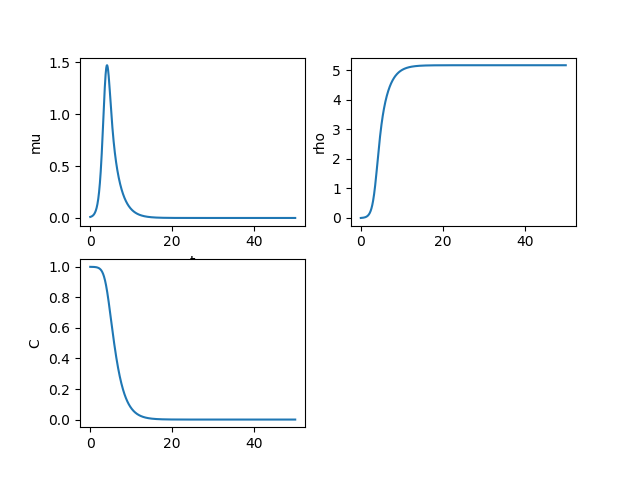
\includegraphics[width=.9\textwidth]{Images/edo_euler_implicite.png}
\caption{Résolution du schéma implicite pour l'EDO}
\end{figure}
 On observe les phénomènes attendus sur l'EDO:\\
 -i) $\mu$ est bornée et tend vers 0.\\
 -ii) $\rho$ est croissante et bornée.\\
 -iii) $C$ décroît vers 0.
\newpage
\subsection{Résolution de l'EDP en 1D}
\subsubsection{Résultat de la simulation de l'EDP en 1D}
\begin{figure}[hbt!]
\centering
\begin{subfigure}[b]{0.45\textwidth}
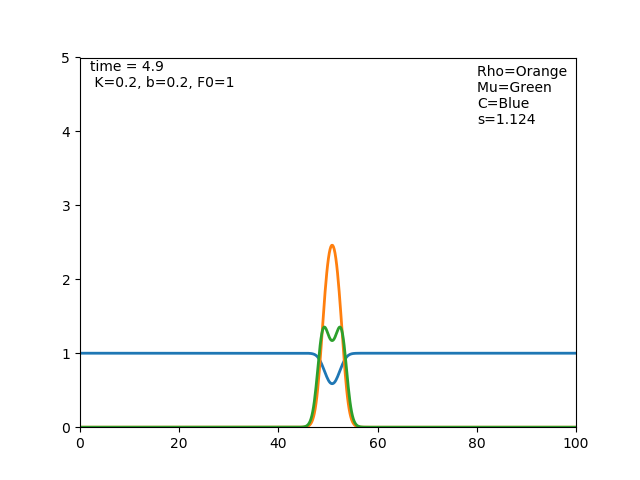
\includegraphics[width=\textwidth]{Images/edp_1d_0.png}
\end{subfigure}
\begin{subfigure}[b]{0.45\textwidth}
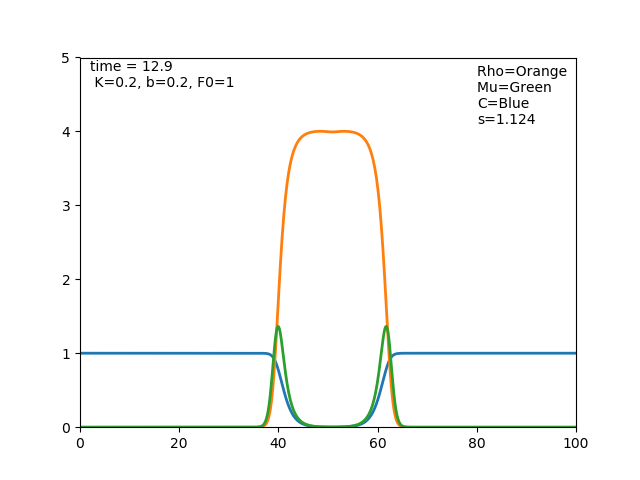
\includegraphics[width=\textwidth]{Images/edp_1d_1.png}
\end{subfigure}
\begin{subfigure}[b]{0.45\textwidth}
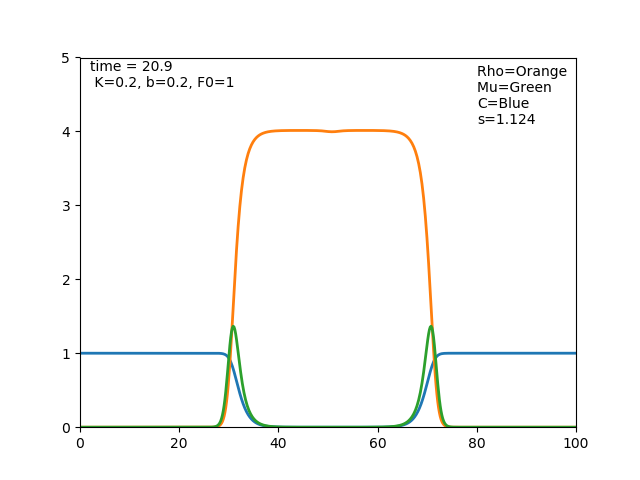
\includegraphics[width=\textwidth]{Images/edp_1d_2.png}
\end{subfigure}
\begin{subfigure}[b]{0.45\textwidth}
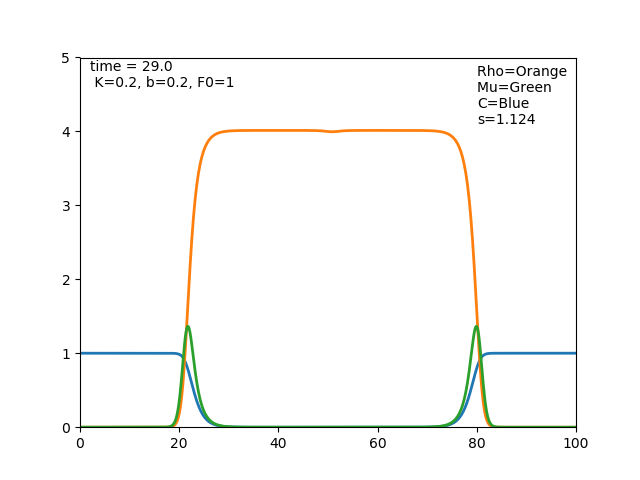
\includegraphics[width=\textwidth]{Images/edp_1d_3.png}
\end{subfigure}
\caption{Résolution du schéma semi implicite I pour l'EDP en 1D} 
\end{figure}
On voit sur les simulations que la solution tend vers une solution de type onde plane stationnaire. Il est possible de calculer cette vitesse et de la comparer avec la vitesse théorique minimale obtenue dans la partie 3: 

\newpage
 
\begin{figure}[hbt!]
\centering
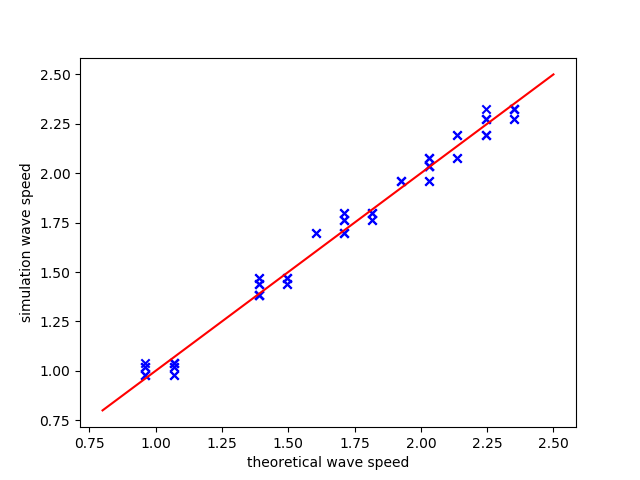
\includegraphics[width=.7\textwidth]{Images/stheoriquevssimulations.png}
\caption{Vitesse du front observée numériquement en fonction de la vitesse minimale théorique}
\end{figure}
Soit \begin{equation*}
s^*_{theorique} =K\frac{f_0(18F_0+4)+\sqrt{f_0(f_0(18F_0+4)^2+108(f_0+4F_0)F_0^2)}}{2(f_0+4F_0)}\end{equation*} la vitesse minimale théorique obtenue dans la partie 3.\\
Ce graphe représente par les points bleus la vitesse du front observée numériquement pour différentes simulations en fonction de la vitesse minimale théorique associée à cette simulation. La droite rouge est la droite $s_{simu} = s^*_{theorique}$.\\
On remarque que la vitesse du front observée numériquement est très proche de la vitesse minimale théorique: ce phénomène est similaire à celui de l'équation de Fisher-KPP: pour une donnée initiale à support compact, \textbf{le front se propage asymptotiquement à la vitesse minimale de l'équation d'onde associée à l'EDP}. %4 et 5
\newpage
\ifdefined\COMPLETE
\else
\documentclass[11pt]{article}
\usepackage[french, english]{babel}
\usepackage[utf8]{inputenc}
\usepackage{graphicx}
\usepackage{framed}
\usepackage[normalem]{ulem}
\usepackage{amsmath}
\usepackage{amsthm}
\usepackage{amssymb}
\usepackage{amsfonts}
\usepackage{enumerate}
\usepackage{import}
\usepackage[top=1 in,bottom=1in, left=1 in, right=1 in]{geometry}
\usepackage{listingsutf8}
\usepackage{color}
\usepackage{float}
\usepackage{graphicx}
\usepackage{subcaption}
\usepackage[toc,page]{appendix}
\usepackage{multicol}
\usepackage{wrapfig}
\usepackage{sidecap}

\floatstyle{boxed} 
\restylefloat{figure}
\definecolor{mygreen}{rgb}{0,0.6,0}
\definecolor{mygray}{rgb}{0.5,0.5,0.5}
\definecolor{mymauve}{rgb}{0.58,0,0.82}
\newcommand{\dt}{\partial_t}
\newcommand{\Tl}{\frac{T}{\lambda}}
\theoremstyle{definition}
\newtheorem{definition}{Définition}[section]
\DeclareMathOperator*{\argmax}{arg\,max}
\DeclareMathOperator*{\argmin}{arg\,min}
 


\lstset{ 
  backgroundcolor=\color{white},   % choose the background color; you must add \usepackage{color} or \usepackage{xcolor}; should come as last argument
  basicstyle=\footnotesize,        % the size of the fonts that are used for the code
  breakatwhitespace=false,         % sets if automatic breaks should only happen at whitespace
  breaklines=true,                 % sets automatic line breaking
  captionpos=b,                    % sets the caption-position to bottom
  commentstyle=\color{mygreen},    % comment style
  deletekeywords={...},            % if you want to delete keywords from the given language
  escapeinside={\%*}{*)},          % if you want to add LaTeX within your code
  extendedchars=true,              % lets you use non-ASCII characters; for 8-bits encodings only, does not work with UTF-8
  firstnumber=1000,                % start line enumeration with line 1000
  frame=single,	                   % adds a frame around the code
  keepspaces=true,                 % keeps spaces in text, useful for keeping indentation of code (possibly needs columns=flexible)
  keywordstyle=\color{blue},       % keyword style
  language=Python,                 % the language of the code
  morekeywords={*,...},            % if you want to add more keywords to the set
  numbers=left,                    % where to put the line-numbers; possible values are (none, left, right)
  numbersep=5pt,                   % how far the line-numbers are from the code
  numberstyle=\tiny\color{mygray}, % the style that is used for the line-numbers
  rulecolor=\color{black},         % if not set, the frame-color may be changed on line-breaks within not-black text (e.g. comments (green here))
  showspaces=false,                % show spaces everywhere adding particular underscores; it overrides 'showstringspaces'
  showstringspaces=false,          % underline spaces within strings only
  showtabs=false,                  % show tabs within strings adding particular underscores
  stepnumber=2,                    % the step between two line-numbers. If it's 1, each line will be numbered
  stringstyle=\color{mymauve},     % string literal style
  tabsize=2,	                   % sets default tabsize to 2 spaces
  title=\lstname                   % show the filename of files included with \lstinputlisting; also try caption instead of title
}
\lstset{inputencoding=utf8/latin1}
\newcommand{\Dt}{\Delta t}
\newcommand{\Dx}{\Delta x}
 %file containing all the used libraries
\newtheorem{theorem}{Théorème}
\begin{document}
\fi
\section{Recherche de la vitesse d'onde des solutions progressives de l'Équation fluide complète du champignon.}
Le but de cette section est de montrer comment l'on peut obtenir la vitesse d’onde pour l’équation du champignon complète:  
\begin{equation}  \left\{
                \begin{array}{ll}
                \dt\mu + \nabla(\mu v) = f(C)(\mu + \rho) -\mu\rho \\
                   \dt(\mu v)+\nabla(\mu v\times v) +T\nabla\mu=-\lambda\mu v+\mu\nabla C-\mu v \rho \\
                 \dt\rho=  F(v) \mu \\
                  \dt C = -b\rho C.
                \end{array}
              \right.
\end{equation} 
En effet dans les sections précédentes nous avons travaillés dans le cas $\lambda$ et $T$ très grands ce qui simplifiait les équations.\\
Cependant nous avons pu voir que, comme pour l’équation de Fisher KPP, pour une donnée initiale à support compact, la solution tend vers une solution d'onde et que la vitesse d'onde peut être retrouvée grâce a la linéarisation autour de l'état initial.\\
Nous allons alors adopter la même stratégie pour l’équation complète.\\
Ici nous allons linéariser autour de l’état $(\mu,\rho,C,v) = (0,0,C_0,v)$.\\
Équation d'onde pour le fluide:\\
Soit $s$ la vitesse d'onde, $y=x-st$, par le même argument de symétrie que pour l’équation de  ``KPP avec mémoire", nous allons se placer dans le cas $s<0$. Avec abus de notation $ :(x,t) = :(y)$, où $y=x-st$, l’équation d'onde pour le fluide est:
\begin{equation}\label{eq:FWS_BDNG}  \left\{
                \begin{array}{ll}
                -s\mu' + (\mu v)' = f(C)(\mu + \rho) -\mu\rho \\
                   -s (\mu v)'+(\mu v\times v)' +T\mu'=-\lambda\mu v+\mu C'-\mu v \rho \\
                 -s \rho '=  F(v) \mu \\
                  -sC' = -b\rho C.
                \end{array}
              \right.
\end{equation} 
Linéarisation autour de l’état  $(\mu,\rho,C,v) = (0,0,C_0,v)$: \\
On pose $f(C_0) = f_0$, et on cherche des solutions de la forme $\rho = \rho_0 \exp(Xy)$ autour de $\rho=0$.\\ 
On obtient en intégrant la quatrième ligne $C= C_0 - \frac{b\rho_0 C_0}{X}\exp(Xy).$\\
La troisième ligne donne: $-sX\rho_0\exp(Xy)=F_0\mu$ donc $\mu = \frac{-sX\rho_0}{F_0}\exp(Xy)$.\\
Autour de $(\mu,\rho,C,v) = (0,0,C_0,v)$, la première ligne donne: $-s\mu' + (\mu v)' = f_0(\mu + \rho)$ car on peut négliger $\mu\rho$ devant $\mu$ et $\rho$ . On a donc \begin{equation}
	(\mu v)'=(f_0\rho_0-\frac{sXf_0\rho_0}{F_0}-\frac{s^2X^2\rho_0}{F_0})\exp(Xy)
\end{equation}
donc \begin{equation}
	\mu v = (\frac{f_0\rho_0}{X}- \frac{f_0s\rho_0}{F_0}-\frac{s^2X\rho_0}{F_0})\exp(Xy).
\end{equation}
Ainsi \begin{equation}
	v= \frac{\mu v}{\mu} = v_0 = s + \frac{f_0}{X}-\frac{f_0F_0}{X^2s}  .
\end{equation}
La deuxième ligne donne $-s (\mu v)'+(\mu v\times v)' +T\mu'=-\lambda\mu v+\mu C'-\mu v \rho$. \\
On peut ici négliger $\mu v\rho$ et $\mu C'$ devant $\mu v$. On a donc: \begin{equation}
	(-v_0sX\mu_0 + v_0^2X\mu_0 +T\mu_0X)\exp(Xy) = -\lambda\mu_0v_0\exp(Xy)
\end{equation}
donc \begin{equation}
	-sXv_0 + v_0^2X+ TX = -\lambda v_0.
\end{equation}
En multipliant par $X^2$ et en substituant $v_0 =  s + \frac{f_0}{X}-\frac{f_0F_0}{X^2s}$ on a alors l’équation caractéristique:
\begin{equation} \label{eq:P}
	X^4(Ts^2) + X^3(\lambda + f_0)s^3+ X^2(f_0^2s^2+ \lambda f_0 s^2 - f_0F_0s^2)+ X(-sF_0f_0)(\lambda+2f_0) + f_0^2F_0^2=0.
\end{equation}
En posant $Y = sX$ on obtient: \begin{equation}
	A(Y) \equiv Y^4+\frac{s^2}{T}P_3(Y)=0 \label{eq:PY}
\end{equation} où \begin{equation}
		P_3(Y) \equiv  Y^3(\lambda + f_0)+ Y^2(f_0^2+ \lambda f_0 - f_0F_0)- Y(F_0f_0(\lambda+2f_0)) + f_0^2F_0^2
\end{equation} est un polynôme de degré 3 dont les coefficients ne dépendent que des données $f_0$, $F_0$, $\lambda$ et $T$. \\
\subsection{Condition d'existence de racines toutes réelles}
La vitesse recherchée est le plus petit $s>0$ (ou plus grand $s<0$ ) tel que le polynôme de degré 4 $A$ défini dans \ref{eq:PY} possède quatre racines réelles (comptées avec multiplicité).\\ 
Effectuons le changement de variable $Y= Y-\frac{b}{4}$ où $b$ est le coefficient devant $Y^3$ dans $A$ et posons $S= \frac{s^2}{T}>0$.\\
 Ce nouveau polynôme (noté $B$) s'écrit: \begin{equation}
	B(Y) \equiv A(Y-\frac{b}{4}) = Y^4 + qY^2 + r Y + \sigma.
\end{equation}
$B$ est dénommé le polynôme réduit de $A$ : on a annulé le terme en $Y^3$.
Pour que $B$ ait 4 racines réelles, les coefficients de $B$ doivent satisfaire trois conditions (de façon nécessaire et suffisante) CITER EQUATION D'ORDRE 4:\\
i) $q<0$,\\
ii) $q^2-4\sigma>0$,\\
iii) Le discriminant $\Delta_B$ de $B$ est positif: $\Delta_B>0$.\\
Les calculs étant très lourds, j'ai utilisé un module de calcul formel pour les effectuer et trouver des factorisations et simplifications. Dans toute la suite, comme $S= \frac{s^2}{T}$, on s’intéressera aux conditions dans le cas $S>0$.
\subsubsection{Condition $q<0$}
On a \begin{equation} q = - \frac{S \left( S \left(3 \lambda^{2} + 6 \lambda f_{0} + 3 f_{0}^{2}\right)+ 8 F_{0} f_{0} + - 8 \lambda f_{0} - 8 f_{0}^{2}\right)}{8}. \end{equation}
Ainsi on a $q<0$ sur un domaine de la forme $[a,\infty[$. Ce domaine est illustré dans la sous-section récapitulative suivante.

\newpage
\subsubsection{Condition $q^2 -4\sigma>0$}
Le calcul formel donne:
\begin{multline}
 q^2 - 4\sigma= S^{3}  \left( \frac{3  \lambda^{4}}{16} +  \frac{3  \lambda^{3} f_{0}}{4} +  \frac{9  \lambda^{2} f_{0}^{2}}{8} +  \frac{3  \lambda f_{0}^{3}}{4} +  \frac{3 f_{0}^{4}}{16} \right) \\ + S^{2}  \left(F_{0}  \lambda^{2} f_{0} + 2 F_{0}  \lambda f_{0}^{2} + F_{0} f_{0}^{3} -  \lambda^{3} f_{0} - 3  \lambda^{2} f_{0}^{2} - 3  \lambda f_{0}^{3} - f_{0}^{4} \right) \\+ S  \left(F_{0}^{2} f_{0}^{2} - F_{0}  \lambda^{2} f_{0} - 5 F_{0}  \lambda f_{0}^{2} - 4 F_{0} f_{0}^{3} +  \lambda^{2} f_{0}^{2} + 2  \lambda f_{0}^{3} + f_{0}^{4} \right)- 4 F_{0}^{2} f_{0}^{2} .
\end{multline}
En particulier c'est un polynôme de degré 3, de coefficient dominant positif, et négatif en $0$.\\ Il admet donc une ou trois racines strictement positives. \\ Dans le premier cas, on a $q^2 -4\sigma>0$ sur un domaine de la forme $[b,\infty[$ et dans le deuxième cas $[b,c[\cup [d,+\infty[ $. Ces cas et ces domaines sont illustrés dans la sous-section récapitulative suivante.


\subsubsection{Condition $\Delta_B >0$}
Le calcul formel montre que $\Delta_B$ s’écrit de la forme: \begin{equation}
	\Delta_B = S^3 L(S)
\end{equation}
où $L$ est un polynôme de degré au plus 3 en $S$. \\
Plus particulièrement:\\
- Son coefficient en $S^3 $ est égal à: \begin{equation}
	F_{0}^{2} f_{0}^{3} \left(4 F_{0} + f_{0} \right)  \left( \lambda + f_{0} \right)^{2}  \left(F_{0} f_{0} -  \lambda^{2} -  \lambda f_{0} \right)^{2} \geq 0
\end{equation} 
- Son discriminant $\Delta_L$ est égal à: \begin{multline} \Delta_L =16 F_{0}^{12} \lambda^{2} f_{0}^{15} \left(4 F_{0} f_{0} - \lambda^{2} - 2 \lambda f_{0}\right)^{2}\\ (32 F_{0}^{3} f_{0}^{2} + 9 F_{0}^{2} \lambda^{2} f_{0} + 48 F_{0}^{2} \lambda f_{0}^{2} + 48 F_{0}^{2} f_{0}^{3} + 27 F_{0} \lambda^{4} + 63 F_{0} \lambda^{3} f_{0} + 60 F_{0} \lambda^{2} f_{0}^{2} + 48 F_{0} \lambda f_{0}^{3} \\ + 24 F_{0} f_{0}^{4} + 9 \lambda^{4} f_{0} + 22 \lambda^{3} f_{0}^{2} + 21 \lambda^{2} f_{0}^{3} + 12 \lambda f_{0}^{4} + 4 f_{0}^{5})^{3} \geq 0 \end{multline}
Donc $\Delta_L \geq 0 $ et donc $L$ a trois racines.\\
- Son terme de degré nul $L(0)=256f_0^6F_0^6$ est positif: $L(0)>0$.\\
Ainsi $\Delta_B$ a zéro ou deux racines strictement positives, ce qui donne dans le premier cas un domaine de vitesse possible de la forme $[0,\infty[$ pour cette condition et dans le deuxième cas $[0,e[\cap[f,+\infty[.$ Ces cas et ces domaines sont illustrés dans la sous-section récapitulative suivante.
\subsubsection{Domaine des vitesses possibles et existence d'une vitesse minimale}
La deuxième condition montre en particulier l'existence d'une vitesse minimale strictement positive (en valeur absolue) de propagation. 
Le domaine du carré des vitesses possible étant l'intersection des trois domaines relatifs aux conditions, il est de la forme:
\begin{equation}
	\mathcal{D}=[a,b[\cap[c,d[\cap[e,+\infty[ \text{ ou } \mathcal{D}=[a,b[\cap[c,+\infty[ \text{ ou } \mathcal{D}=[a,+\infty[
\end{equation}
où $0<a<b<c<d<e$.\\
\newpage
\subsubsection{Récapitulatif et discussion graphique des trois conditions.}
Partout, la zone $S<0$ est invalide (rouge) car $S=\frac{s^2}{T}>0$.\\
Le domaine des vitesses possible est alors l'intersection des domaines valides (verts) pour les trois conditions:

i) Deux cas possibles sur la condition $q(S)<0$:\\


\begin{tabular}{cc}
 La racine de $q/S$ est positive & La racine de $q/S$ est négative \\
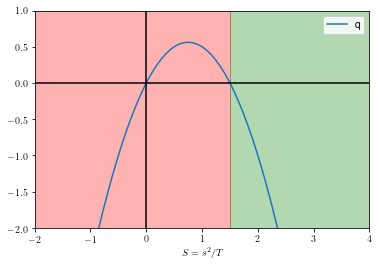
\includegraphics[width=.47\textwidth]{Images/qcas1.png} & 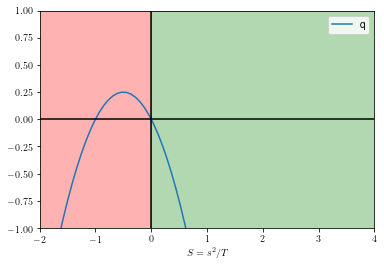
\includegraphics[width=.47\textwidth]{Images/qcas2.png} \\
\end{tabular}
\\
ii) Deux cas possibles sur la condition $q(S)^2-4\sigma(S)>0$:\\

\begin{tabular}{cc}
Une racine positive. & Trois racines positives. \\
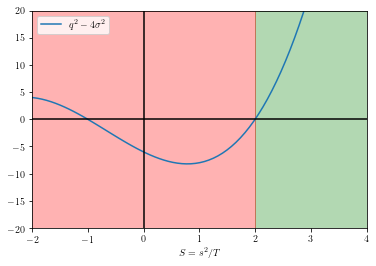
\includegraphics[width=.47\textwidth]{Images/q2cas1.png} & 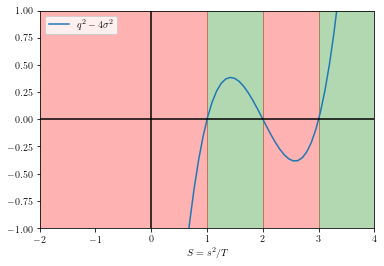
\includegraphics[width=.47\textwidth]{Images/q2cas2.png} \\
\end{tabular}
iii) Deux cas possibles sur la condition $\Delta_A(S) >0$:\\

\begin{tabular}{cc}
Trois racines négatives. & Une racine négative et deux positives.\\
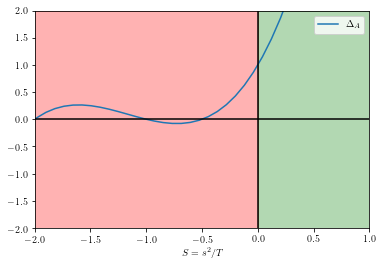
\includegraphics[width=.47\textwidth]{Images/deltacas1.png} & 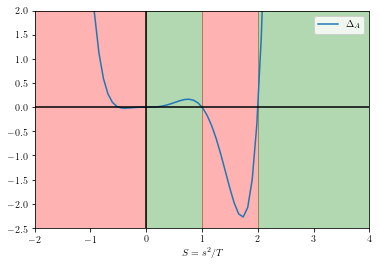
\includegraphics[width=.47\textwidth]{Images/deltacas2.png} \\
\end{tabular}






\subsection{Condition d'amortissement et détermination de la vitesse d'onde sélectionnée}
Lors des simulations, on s’aperçoit que la vitesse d'onde sélectionnée n'est pas pour tous les paramètres $\lambda,f_0,F_0,T$ le plus petit $s$ tel que le polynôme $A$ admet 4 racines réelles (condition de régime apériodique en physique) . Une autre condition apparaît: le $s$ cherché est la plus petite vitesse d'onde positive (ou la plus grande négative) tel que la linéarisation autour de l’état $(\mu,\rho,C,v) = (0,0,C_0,v_0)$ satisfait une condition dite "d'amortissement" (qui sera analogue a la condition de régime critique en physique).
\begin{definition}{\textbf{Condition d'amortissement}} \\ Un polynôme $P \in \mathbb{R}[X]$ est dit satisfaire la condition d'amortissement pour notre problème si sa racine de plus petite partie réelle négative est réelle.
\end{definition}

La condition d'amortissement pour un polynôme montre que la dynamique de l'EDO liée au polynôme
\begin{theorem}\textbf{{Condition d'amortissement et positivité} }\\
$P$ vérifie la condition d'amortissement si et seulement si l'EDO associée à P ne s'annule pas autour de $-\infty$ pour des données initiales positives.
\end{theorem}
\begin{proof}Si $P$ vérifie la condition d'amortissement, soit alors $r_1$ la racine de plus petite partie réelle de $P$: elle est réelle. \\ 
Les solutions de l'EDO associé à $P$ avec conditions initiales positives sont de la forme: \begin{equation}
	f(x)=A_1\exp(r_1x)+ \sum_{i>1,r_i\in\mathbb{R}}(A_i\exp(r_ix)) + \sum_{i>1,r_i\not\in\mathbb{R}}B_i\exp(\Re(r_i))\cos(\omega_it)
\end{equation}
En particulier quand $x\to -\infty$, $f(x)\sim  A_1\exp(r_1x) >0$.\\
Réciproquement, les solutions $f$ de l'EDO sont équivalentes à $A_i\exp(\Re(r_i))cos(\omega_it)$, où $r_i$ est la racine de plus petite partie réelle. Pour ne pas avoir d’annulation, il faut $\omega_i =0 $ donc $r_i \in \mathbb{R}.$
\end{proof}


\subsubsection{Recherche de la vitesse d'onde extrémale satisfaisant la condition d'amortissement}
Soit $Y$ une racine du polynôme A défini \ref{eq:PY}, $s$ est déterminé par $Y$ par l'équation: \begin{equation}
	s^2 = -\frac{TY^4}{P_3(Y)}. \label{eq:sfromY}
\end{equation} 
Étudions alors la fonction $ s: Y \mapsto s(Y) = -\sqrt{\frac{TY^4}{P_3(Y)}} $.

\paragraph{Intervalle de définition:}
s(Y) est défini pour tous les $Y$ tels que $P_3(Y)<0$. Étudions alors le polynôme $P_3(Y)=Y^3(\lambda + f_0)+ Y^2(f_0^2+ \lambda f_0 - f_0F_0)- Y(F_0f_0(\lambda+2f_0)) + f_0^2F_0^2$:\\
i) Le coefficient dominant de $P_3$ est positif.\\
ii) Son discriminant est égal à: \begin{equation}
	\Delta_{P_3}= F_{0}^{2} f_{0}^{3} (4 F_{0} + f_{0}) (F_{0} f_{0} -\lambda ^{2} - \lambda  f_{0})^{2} \geq 0.
\end{equation}
Donc $P_3$ a 3 racines réelles (comptées avec multiplicité), notées $r_1\leq r_2 \leq r_3$.\\
iii) Le coefficient constant de $P_3$ est positif donc $-r_1r_2r_3>0$. Donc $r_1<0$, et $r_2$ et $r_3$ sont de même signe. Le coefficient d'ordre 1 de $P_3$ est négatif, donc $r_1r_2 + r_2r_3 + r_1r_3<0$ donc $r_1(r_2+r_3)+r_2r_3<0$ donc $r_2+r_3>0$ donc $r_2>0$ et $r_3>0$. $P_3$ a donc une racine négative et deux racines positives.

\begin{tabular}{cc}
 Polynôme $P_3(Y)$ & Fonction $s(Y) = -\sqrt{\frac{TY^4}{P_3(Y)}}$ \\
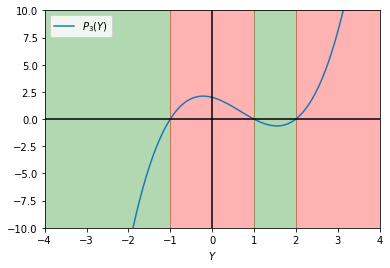
\includegraphics[width=.47\textwidth]{Images/P3.png} & 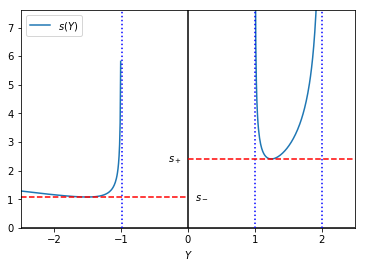
\includegraphics[width=.47\textwidth]{Images/s+s-.png} \\
\end{tabular}

\paragraph{Extremums:} Les extremums de $s$ sont définis par la relation:\begin{equation}
	\frac{\partial s}{\partial Y}=0
\end{equation}
Donc nécessairement: \begin{equation}
	\Big(\frac{Y^4}{P_3(Y)}\Big)'=0
\end{equation} 
i.e. \begin{equation}
\label{eq:Q}	Q(Y)\equiv4P_3(Y)-YP'_3(Y)=0
\end{equation}
Y est alors une racine du polynôme $Q$ défini ci dessus.\\
 Un calcul formel montre que son discriminant $\Delta _Q$ est positif: \begin{multline*}
\Delta _Q = 128F_0^5f_0^5 + 36 F_0^4 \lambda^2 f_0^4 + 192 F_0^4 \lambda f_0^5 + 192 F_0^4 f_0^6 + 108 F_0^3 \lambda^4 f_0^3 + 252 F_0^3 \lambda^3 f_0^4 + 240 F_0^3 \lambda^2 f_0^5 \\+ 192 F_0^3 \lambda f_0^6 + 96 F_0^3 f_0^7 + 36 F_0^2 \lambda^4 f_0^4 + 88 F_0^2 \lambda^3 f_0^5 + 84 F_0^2 \lambda^2 f_0^6 + 48 F_0^2 \lambda f_0^7 + 16 F_0^2 f_0^8 > 0
\end{multline*} donc $Q$ a trois racines.\\
On obtient donc au plus trois extremums pour $s$ par la formule: \begin{equation*}
	s^2 = -\frac{Y^4}{P_3(Y)}.
\end{equation*}
où $Y$ est une racine de $Q$. En fait, on a que deux extremum car l'une de ces racines correspond  au cas $r_1<Y<r_2$ pour le quel $P_3(Y)>0$ et donc $s$ n'est pas défini.\\ Un extremum, noté $s_-$ (correspondant à la plus petite racine de $Q$) appartient au cas $Y<r_1<0$, et l'autre, noté $s_+$ (correspondant à la plus grande racine de $Q$) appartient au cas $0<r_2<Y<r_3$. 
\newpage
\begin{figure}[h!]
\centering
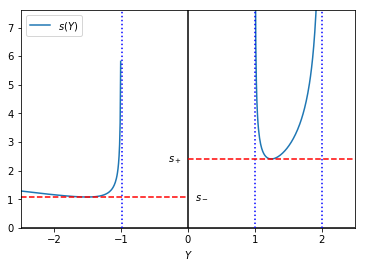
\includegraphics[width=.7\textwidth]{Images/s+s-.png}
\caption{Graphe de la fonction s(Y) et points d’intérêt.}
\end{figure}
On cherche le plus petit $s$, noté $s_{sel}$ tel que la condition d'amortissement sur $A$ soit vérifiée.\\
Pour $s> \max(s_+,s_-)$, $A$ a 4 racines réelles donc la condition d'amortissement est vérifiée.\\
Pour $s< \min(s_+,s_-)$, $A$ n'a pas de racines réelles donc la condition d'amortissement est violée.\\
Ainsi, $ \min(s_+,s_-) \leq s_{sel} \leq \max(s_+,s_-)$.
On va montrer que l'on a toujours $s_{sel} = s_-$: 
\begin{theorem}\textbf{{La plus petite vitesse en valeur absolue pour laquelle la condition d'amortissement est vérifiée correspond à la plus petite racine de $Q$, i.e. $s_{sel}=s_-$}}\\
Soit $s_{sel} =\min \{s>0,\text{Le polynôme $A_s$ vérifie la condition d'amortissement} \}$, i.e. la racines de plus petite partie réelle du polynôme $A_s= Y^4 + \frac{s^2}{T}P_3(Y)$ est réelle.\\
Soit $Q = 4P_3(Y)-YP'_3(Y)$ et soit $y_{min}$ sa plus petite racine (donc négative). Soit $s_- =  \sqrt{\frac{Ty_i^4}{P_3(y_i)}} $.
Alors \boxed{s_- = s_{sel}}
\end{theorem}
\begin{proof} \ \\
On a $ \min(s_+,s_-) \leq s_{sel} \leq \max(s_+,s_-)$.\\
La preuve se fait en deux cas:

\textbf{i) Premier cas:} $s_- < s_+$:\\
Dans ce cas, on sait déjà que $s_{sel} \geq s_-$ .\\
On va alors montrer que $A_{s_-} = Y^4+ \frac{s_-^2}{T}P_3(Y)$, ce qui donnera $s_{sel} \leq s_-$ donc $s_{sel} = s_-$.\\
Soit $Y_{1}$ la plus petite racine de $Q$. Nécessairement, $A_{s_-}$ a une racine double en $Y_1$. \\
Soit alors $Y_2$ et $Y_{3}$ ses deux autres racines. \\
Comme $s_-<s_+$, $Y_2$ et $Y_3$ sont des racines complexe conjuguées.\\ Grace aux relations de Viète (relations coefficients racines), on a:\\
\begin{equation}
	2Y_1 + 2\Re(Y_2) = - \frac{s_-^2}{T}(\lambda + f_0)	
\end{equation}
donc \begin{equation}
	2\Re(Y_2) =  - \frac{s_-^2}{T}(\lambda + f_0)	- 2Y_1.
\end{equation}
Or \begin{equation}
	\frac{s_-^2}{T} = \frac{Y_1^4}{P_3(Y_1)}
\end{equation}  
donc: \begin{align*}
	2\Re(Y_2) &=  - \frac{Y_1^4}{P_3(Y_1)}(\lambda + f_0)	- 2Y_1 \\
	&=- \frac{Y_1}{P_3(Y_1)}((\lambda + f_0)Y_1^3 - 2P_3(Y_1))\\
	&=-\frac{Y_1}{P_3(Y_1)}(Q(Y_1)+F_0f_0(\lambda+2f_0)Y_1 - 2F_0^2f_0^2)
\end{align*}
or $Q(Y_1) = 0$ et $Y_1<0$ et $P_3(Y_1)<0$ donc: \begin{equation}
	\Re(Y_2)>0.
\end{equation}
En particulier $Y_1 < \Re(Y_2)$ donc la racine de plus petite partie réelle est réelle donc $A_{s_-}$ satisfait la condition d'amortissement. Ainsi dans ce cas, \underline{$s_{sel} = s_-$}.\\

\textbf{ii) Deuxième cas:} $s_- > s_+$:\\
Dans ce cas, on sait déjà que $s_{sel} \leq s_{-}$.\\
On va alors montrer que $s_{sel} \geq s_{-}$. Pour cela, on va prendre $s \in [s_{+},s_-[$ et montrer que $A_s$ ne satisfait pas la condition d'amortissement.\\
Soit $s\in [s_{+},s[$.\\
 $A_s$ a deux racines réelles positives $Y_3$ et $Y_4$ et deux racines imaginaires conjuguées $Y_1$ et $Y_2$. \\ 
Montrons que $\Re(Y_1)<0$, ce qui montrera que la racine de plus petite partie réelle est imaginaire et donc $s_{sel} \not = s$.\\
Grace aux relations de Viète (relations coefficients racines), on a:\\
\begin{equation}
	2\Re(Y_1)  =  -Y_3 - Y_4 - \frac{s^2}{T}(\lambda + f_0)	 <0
\end{equation}
Ainsi, $\Re(Y_1)<0<Y_3,Y_4$ et donc $s_{sel} \not = s \ \forall s \in [s_{+},s_-[$. Or $s_sel \in [s_{+},s_-]$ donc \underline{$s_{sel} = s_-$}.\\
\ \\
Ainsi dans nos deux cas, on a \underline{$s_{sel} = s_-$}.

\end{proof}
\ifdefined\COMPLETE
\else
\end{document}
\begin{algorithm}[H]
\SetAlgoLined
\KwResult{Vitesse d'onde extrémale $s$ de l’équation d'onde associée au fluide}
 Entrées: données $\lambda$, $f_0$, $F_0$, $T$ et un $\epsilon$ choisi petit\;
 Calculer les racines réelles $y_i$ du polynôme $Q$ défini par \ref{eq:Q}\; 
 Candidats = $[]$\;
 \For{$y_i$ racine réelle de $Q$}{\If{$P_3(y_i)<0$}{Poser $s_i^2 = -\frac{y_i^4}{P_3(Y_i)}$ avec $s_i<0$\;
 Candidats $+=$ [$s_i$]}
 {}}
 \For{$s_i \in$ Candidats}{\If{le polynôme $Y^4 +(s_i^2-\epsilon)P_3(Y)$ n'a pas 4 racines réelles}{Candidats = Candidats \textbackslash $\{s_i\}$}}
 $s= \max$(Candidats)
 \caption{Recherche de la vitesse d'onde pour l’équation fluide}
\end{algorithm}
\fi

 %6
\newpage
\ifdefined\COMPLETE
\else
\documentclass[11pt]{article}
\usepackage[french, english]{babel}
\usepackage[utf8]{inputenc}
\usepackage{graphicx}
\usepackage{framed}
\usepackage[normalem]{ulem}
\usepackage{amsmath}
\usepackage{amsthm}
\usepackage{amssymb}
\usepackage{amsfonts}
\usepackage{enumerate}
\usepackage{import}
\usepackage[top=1 in,bottom=1in, left=1 in, right=1 in]{geometry}
\usepackage{listingsutf8}
\usepackage{color}
\usepackage{float}
\usepackage{graphicx}
\usepackage{subcaption}
\usepackage[toc,page]{appendix}
\usepackage{multicol}
\usepackage{wrapfig}
\usepackage{sidecap}

\floatstyle{boxed} 
\restylefloat{figure}
\definecolor{mygreen}{rgb}{0,0.6,0}
\definecolor{mygray}{rgb}{0.5,0.5,0.5}
\definecolor{mymauve}{rgb}{0.58,0,0.82}
\newcommand{\dt}{\partial_t}
\newcommand{\Tl}{\frac{T}{\lambda}}
\theoremstyle{definition}
\newtheorem{definition}{Définition}[section]
\DeclareMathOperator*{\argmax}{arg\,max}
\DeclareMathOperator*{\argmin}{arg\,min}
 


\lstset{ 
  backgroundcolor=\color{white},   % choose the background color; you must add \usepackage{color} or \usepackage{xcolor}; should come as last argument
  basicstyle=\footnotesize,        % the size of the fonts that are used for the code
  breakatwhitespace=false,         % sets if automatic breaks should only happen at whitespace
  breaklines=true,                 % sets automatic line breaking
  captionpos=b,                    % sets the caption-position to bottom
  commentstyle=\color{mygreen},    % comment style
  deletekeywords={...},            % if you want to delete keywords from the given language
  escapeinside={\%*}{*)},          % if you want to add LaTeX within your code
  extendedchars=true,              % lets you use non-ASCII characters; for 8-bits encodings only, does not work with UTF-8
  firstnumber=1000,                % start line enumeration with line 1000
  frame=single,	                   % adds a frame around the code
  keepspaces=true,                 % keeps spaces in text, useful for keeping indentation of code (possibly needs columns=flexible)
  keywordstyle=\color{blue},       % keyword style
  language=Python,                 % the language of the code
  morekeywords={*,...},            % if you want to add more keywords to the set
  numbers=left,                    % where to put the line-numbers; possible values are (none, left, right)
  numbersep=5pt,                   % how far the line-numbers are from the code
  numberstyle=\tiny\color{mygray}, % the style that is used for the line-numbers
  rulecolor=\color{black},         % if not set, the frame-color may be changed on line-breaks within not-black text (e.g. comments (green here))
  showspaces=false,                % show spaces everywhere adding particular underscores; it overrides 'showstringspaces'
  showstringspaces=false,          % underline spaces within strings only
  showtabs=false,                  % show tabs within strings adding particular underscores
  stepnumber=2,                    % the step between two line-numbers. If it's 1, each line will be numbered
  stringstyle=\color{mymauve},     % string literal style
  tabsize=2,	                   % sets default tabsize to 2 spaces
  title=\lstname                   % show the filename of files included with \lstinputlisting; also try caption instead of title
}
\lstset{inputencoding=utf8/latin1}
\newcommand{\Dt}{\Delta t}
\newcommand{\Dx}{\Delta x}
 %file containing all the used libraries
\begin{document}
\fi


\section{Appendices}
\subsection{Code de résolution de l'EDO}
\lstinputlisting[language=Python]{edo.py}
\newpage
\subsection{Code de la résolution de l'EDP en 1D}
\lstinputlisting[language=Python]{edp_1d.py}
\newpage
\subsection{Code de la résolution de l'EDP en 2D}
\lstinputlisting[language=Python]{edp_2d.py}

\ifdefined\COMPLETE
\else
\end{document}
\fi

\end{document}